\subsection{Zener Diode:}

Following the Figure 3.1.0, we assembled 3 similar circuits but using different $R_{L}$ and $R_{lim}$ resistors as well different Zener diodes. In each circuit we connected a voltage source in $V_{in}$ varying it from 3.0 to 15 V in intervals of 1 V. All the measures for voltage in $R_{L}$ were registered in the tables below.

\begin{figure}[H]
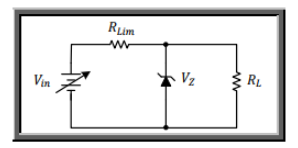
\includegraphics[scale=.8]{d1.png}
\centering \linebreak \linebreak Figure 3.1.0: Zener diode circuit.
\end{figure}

{\bfseries\itshape\color{armygreen}{Observation:}} {\itshape\color{armygreen}{For measure the voltage in $R_{L}$ it's necessary to connect a voltmeter in parallel with the resistor.}}

\begin{multicols}{3}
\begin{tasks}
\task {\bfseries\itshape First circuit:}
\begin{enumerate}
\item Zener Diode: 3.3 V
\item $R_{L}$ resistor: 33 $\Omega$.
\item $R_{lim}$ resistor: 82 $\Omega$.
\end{enumerate}

\begin{center}
\begin{tabular}[.5cm]{ c c }
\toprule
Source Voltage & Voltage in $R_{L}$ \\
\midrule
3.0 V & 0.85 V \\
\cmidrule{1-2}
4.0 V & 1.13 V \\
\cmidrule{1-2}
5.0 V & 1.42 V \\
\cmidrule{1-2}
6.0 V & 1.69 V \\
\cmidrule{1-2}
7.0 V & 1.96 V \\
\cmidrule{1-2}
8.0 V & 2.23 V \\
\cmidrule{1-2}
9.0 V & 2.48 V \\
\cmidrule{1-2}
10.0 V & 2.71 V \\
\cmidrule{1-2}
11.0 V & 2.90 V \\
\cmidrule{1-2}
12.0 V & 3.0 V \\
\cmidrule{1-2}
13.0 V & 3.2 V \\
\cmidrule{1-2}
14.0 V & 3.3 V \\
\cmidrule{1-2}
15.0 V & 3.3 V \\
\bottomrule
\end{tabular}
\end{center} 


\task {\bfseries\itshape Second circuit:}
\begin{enumerate}
\item Zener Diode: 5.1 V
\item $R_{L}$ resistor: 49 $\Omega$.
\item $R_{lim}$ resistor: 56 $\Omega$.
\end{enumerate}

\begin{center}
\begin{tabular}[.5cm]{ c c }
\toprule
Source Voltage & Voltage in $R_{L}$ \\
\midrule
3.0 V & 1.3 V \\
\cmidrule{1-2}
4.0 V & 1.8 V \\
\cmidrule{1-2}
5.0 V & 2.2 V \\
\cmidrule{1-2}
6.0 V & 2.6 V \\
\cmidrule{1-2}
7.0 V & 3.1 V \\
\cmidrule{1-2}
8.0 V & 3.5 V \\
\cmidrule{1-2}
9.0 V & 4.0 V \\
\cmidrule{1-2}
10.0 V & 4.4 V \\
\cmidrule{1-2}
11.0 V & 4.9 V \\
\cmidrule{1-2}
12.0 V & 5.1 V \\
\cmidrule{1-2}
13.0 V & 5.2 V \\
\cmidrule{1-2}
14.0 V & 5.2 V \\
\cmidrule{1-2}
15.0 V & 5.3 V \\
\bottomrule
\end{tabular}
\end{center}

\task {\bfseries\itshape Third circuit:}
\begin{enumerate}
\item Zener Diode: 9.1 V
\item $R_{L}$ resistor: 82 $\Omega$.
\item $R_{lim}$ resistor: 27 $\Omega$.
\end{enumerate}

\begin{center}
\begin{tabular}[.5cm]{ c c }
\toprule
Source Voltage & Voltage in $R_{L}$ \\
\midrule
3.0 V & 2.2 V \\
\cmidrule{1-2}
4.0 V & 2.9 V \\
\cmidrule{1-2}
5.0 V & 3.7 V \\
\cmidrule{1-2}
6.0 V & 4.5 V \\
\cmidrule{1-2}
7.0 V & 5.3 V \\
\cmidrule{1-2}
8.0 V & 6.0 V \\
\cmidrule{1-2}
9.0 V & 6.7 V \\
\cmidrule{1-2}
10.0 V & 7.4 V \\
\cmidrule{1-2}
11.0 V & 8.1 V \\
\cmidrule{1-2}
12.0 V & 8.7 V \\
\cmidrule{1-2}
13.0 V & 9.0 V \\
\cmidrule{1-2}
14.0 V & 9.2 V \\
\cmidrule{1-2}
15.0 V & 9.3 V \\
\bottomrule
\end{tabular}
\end{center}
\end{tasks}
\end{multicols}


\pagebreak